\documentclass[11pt,preprint, authoryear]{article}

\pagestyle{plain}

\usepackage{lmodern}
%%%% My spacing
\usepackage{setspace}
\setstretch{1.5}
\DeclareMathSizes{10}{12}{8}{8}

% Wrap around which gives all figures included the [H] command, or places it "here". This can be tedious to code in Rmarkdown.
\usepackage{float}
\let\origfigure\figure
\let\endorigfigure\endfigure
\renewenvironment{figure}[1][2] {
    \expandafter\origfigure\expandafter[H]
} {
    \endorigfigure
}

\let\origtable\table
\let\endorigtable\endtable
\renewenvironment{table}[1][2] {
    \expandafter\origtable\expandafter[H]
} {
    \endorigtable
}


\usepackage{ifxetex,ifluatex}
\usepackage{fixltx2e} % provides \textsubscript
\ifnum 0\ifxetex 1\fi\ifluatex 1\fi=0 % if pdftex
  \usepackage[T1]{fontenc}
  \usepackage[utf8]{inputenc}
\else % if luatex or xelatex
  \ifxetex
    \usepackage{mathspec}
    \usepackage{xltxtra,xunicode}
  \else
    \usepackage{fontspec}
  \fi
  \defaultfontfeatures{Mapping=tex-text,Scale=MatchLowercase}
  \newcommand{\euro}{€}
\fi

\usepackage{amssymb, amsmath, amsthm, amsfonts}

\usepackage[round]{natbib}
\bibliographystyle{natbib}
\def\bibsection{\section*{References}} %%% Make "References" appear before bibliography
\usepackage{longtable}
\usepackage[margin=2cm,bottom=4cm,top=2.5cm, includefoot]{geometry}
\usepackage{fancyhdr}
\usepackage[bottom, hang, flushmargin]{footmisc}
\usepackage{graphicx}
\numberwithin{equation}{section}
\numberwithin{figure}{section}
\numberwithin{table}{section}
\setlength{\parindent}{0cm}
\setlength{\parskip}{1.3ex plus 0.5ex minus 0.3ex}
\usepackage{textcomp}
\renewcommand{\headrulewidth}{0pt}

\usepackage{array}
\newcolumntype{x}[1]{>{\centering\arraybackslash\hspace{0pt}}p{#1}}

%%%%  Remove the "preprint submitted to" part. Don't worry about this either, it just looks better without it:

\makeatletter
\def\ps@pprintTitle{%
  \let\@oddhead\@empty
  \let\@evenhead\@empty
  \let\@oddfoot\@empty
  \let\@evenfoot\@oddfoot
}

\usepackage{hyperref}
\hypersetup{breaklinks=true,
            bookmarks=true,
            colorlinks=true,
            citecolor=blue,
            urlcolor=blue,
            linkcolor=blue,
            pdfborder={0 0 0}}
						
\urlstyle{same}  % don't use monospace font for urls
\setlength{\parindent}{0pt}
\setlength{\parskip}{6pt plus 2pt minus 1pt}
\setlength{\emergencystretch}{3em}  % prevent overfull lines
\setcounter{secnumdepth}{5}

%%% Use protect on footnotes to avoid problems with footnotes in titles
\let\rmarkdownfootnote\footnote%
\def\footnote{\protect\rmarkdownfootnote}
\IfFileExists{upquote.sty}{\usepackage{upquote}}{}

%%% Include extra packages specified by user
\usepackage{amsmath}

%%% Change title format to be more compact
\usepackage{titling}

% Create subtitle command for use in maketitle
%\newcommand{\subtitle}[1]{
  %\posttitle{
    %\begin{center}\large#1\end{center}
    %}
%}

\setlength{\droptitle}{-1em}
\title{Department of Statistics 2019: Mapping Inequalities Online Using GitHub
Data}
\pretitle{\vspace{\droptitle}\centering\huge}
\posttitle{\par\vskip 0.5em}
\author{Candidate Number: 10140}
\preauthor{\centering\large}
\postauthor{\par}
\predate{\centering\large}
\postdate{\par}
\date{}

\usepackage{color}
\usepackage[usenames,dvipsnames,svgnames,table]{xcolor}
\usepackage{hyperref}
\hypersetup{
     colorlinks   = true,
     citecolor    = gray
}

\usepackage{tocloft}

\renewcommand{\cftsubsecfont}{\normalfont\hypersetup{linkcolor=black}}
\renewcommand{\cftsubsecafterpnum}{\hypersetup{linkcolor=black}}

\begin{document}

%________________________
% Header and Footers
%%%%%%%%%%%%%%%%%%%%%%%%%%%%%%%%%
\pagestyle{fancy}
\chead{}
\rhead{}
\lfoot{}
\rfoot{} 
\lhead{}
%\rfoot{\footnotesize Page \thepage\ } % "e.g. Page 2"
\cfoot{\footnotesize \thepage\\}

%\setlength\headheight{30pt} 
%%%%%%%%%%%%%%%%%%%%%%%%%%%%%%%%%
%________________________

%\headsep 35pt % So that header does not go over title

%\begin{frontmatter}

\pagenumbering{roman}



\maketitle
\thispagestyle{empty}

%\author{Candidate Number: 10140}
%\date{}


%\end{frontmatter}

\clearpage

\setcounter{page}{1}

\renewcommand{\contentsname}{Contents}
\hypersetup{linkcolor=black}
\tableofcontents
\newpage
\hypersetup{linkcolor=black}
\listoftables
\newpage
\hypersetup{linkcolor=black}
\listoffigures
\hypersetup{linkcolor=black}
\newpage

\pagenumbering{arabic}

\renewcommand{\vec}[1]{\mathbf{#1}}


\section{\texorpdfstring{Introduction
\label{Intro}}{Introduction }}\label{introduction}

\newpage

\section{\texorpdfstring{Brief Literature Review
\label{Lit}}{Brief Literature Review }}\label{brief-literature-review}

\subsection{A Summary of the Research}\label{a-summary-of-the-research}

Brinton \emph{et al.} (2014)

Stadtfeld \emph{et al.} (2019)

Currarini, Jackson and Pin (2010)

\newpage

\section{\texorpdfstring{Datasets I Have Found
\label{Data}}{Datasets I Have Found }}\label{datasets-i-have-found}

\newpage

\section{\texorpdfstring{Empirical Methodology
\label{Meth}}{Empirical Methodology }}\label{empirical-methodology}

\subsection{\texorpdfstring{Empirical Model
\label{Model}}{Empirical Model }}\label{empirical-model}

This is an equation:

\begin{align} \label{eq:EP1}
A_{it}=f(T_i^{(t)},S_i^{(t)},P_i^{(t)},B_i^{(t)},I_i),
\end{align}

\footnotesize
\renewcommand{\thetable}{\arabic{table}}

\begin{longtable} {@{} l r r c r @{}} \caption{\textbf{Learner achievement (\%)}}
\label{tab:Dep}\\ \hline \hline
Subject & Mean & Q1 & Median & Q3 \\
\hline
Maths&      27& 15&   23&  35\\ \hline \hline
\end{longtable}\begin{center} Source: Own calculations in Stata using 2004 Grade 6 Intermediate Phase Systemic Evaluation.\end{center}

\normalsize

\setcounter{figure}{0} \renewcommand{\thefigure}{\arabic{figure}}

\begin{figure}
\caption{\textbf{\footnotesize Cumulative graph for subject scores}}
\label{fig:1}

\begin{center}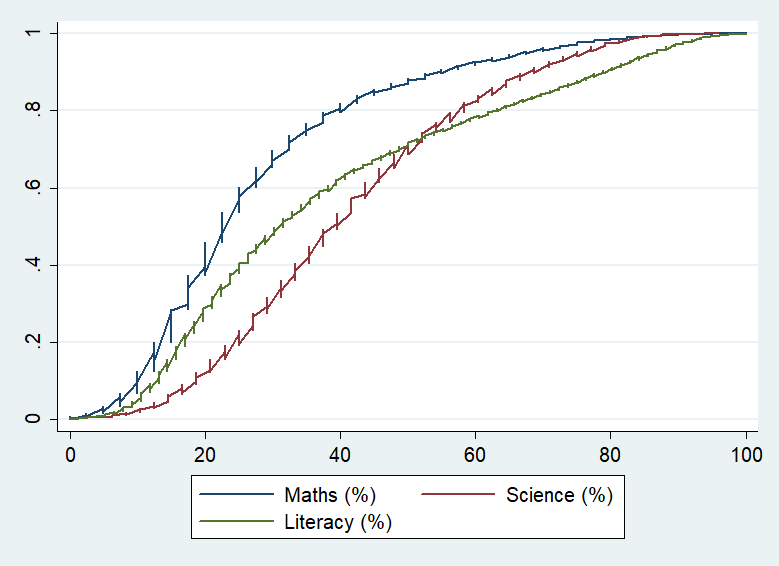
\includegraphics[width=0.4\linewidth]{./results/graphs/figure} \end{center}
\centering
{\footnotesize Source: Own calculations in Stata using 2004 Grade 6 Intermediate Phase Systemic Evaluation.}
\end{figure}

\normalsize

Again, you can reference the figure in-text: figure \ref{fig:1} is a
figure and it displays etc. etc. etc.

This is an organic figure generated with an R chunk that is executed
when the document is knitted (the image is also saved in the folder
\texttt{final-article-template\_files}):

\begin{center}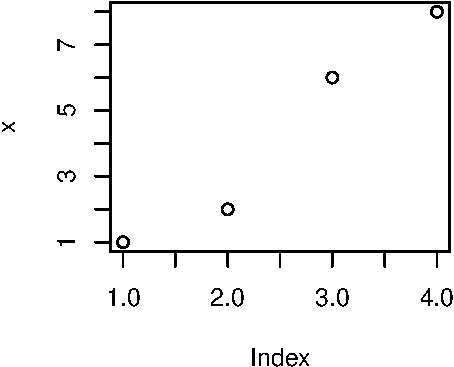
\includegraphics[width=0.4\linewidth]{final-msc-article_files/figure-latex/unnamed-chunk-2-1} \end{center}

Regarding R chunks: If you want a chunk's code to be printed, include
set \texttt{echo\ =\ TRUE}. \texttt{message\ =\ FALSE} stops R printing
package loading details and setting \texttt{warning\ =\ FALSE} should
suppress most warnings.

\newpage

\section{\texorpdfstring{Recommendations for Further Research
\label{Recom}}{Recommendations for Further Research }}\label{recommendations-for-further-research}

\newpage

\section{\texorpdfstring{Concluding Remarks
\label{Concl}}{Concluding Remarks }}\label{concluding-remarks}

\newpage

\section{References}\label{references}

\hypertarget{refs}{}
\hypertarget{ref-Brinton2014}{}
Brinton, C. G. \emph{et al.} (2014) `Learning about social learning in
MOOCs: From statistical analysis to generative model', \emph{IEEE
Transactions on Learning Technologies}. IEEE, 7(4), pp. 346--359. doi:
\href{https://doi.org/10.1109/TLT.2014.2337900}{10.1109/TLT.2014.2337900}.

\hypertarget{ref-Currarini2010}{}
Currarini, S., Jackson, M. O. and Pin, P. (2010) `Identifying the roles
of race-based choice and chance in high school friendship network
formation', \emph{Proceedings of the National Academy of Sciences},
107(11), pp. 4857--4861. doi:
\href{https://doi.org/10.1073/pnas.0911793107}{10.1073/pnas.0911793107}.

\hypertarget{ref-Stadtfeld2019}{}
Stadtfeld, C. \emph{et al.} (2019) `Integration in emerging social
networks explains academic failure and success', 116(3), pp. 792--797.
doi:
\href{https://doi.org/10.1073/pnas.1811388115}{10.1073/pnas.1811388115}.

\newcommand\wordcount{
    \immediate\write18{texcount -sub=section \jobname.tex  | grep "Section" |     sed -e 's/+.*//' | sed -n \thesection p > 'count.txt'}
(\input{count.txt}words)}

\section*{References}

\end{document}
